\scanpage{42}
\margin{\unsure{Commencer}\par\unsure{Voir ça}\par\unsure{Voir} \unsure{dans le livre de} \illegible{1}\par\unsure{puis au corollaire}}
\figure{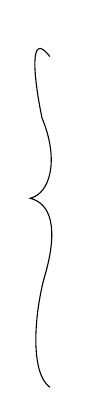
\begin{tikzpicture}[x=.25cm,y=.6cm]\draw (1,8) .. controls (-.1,8.6) and (.2,7.5) .. (.6,6.7) .. controls (1.5,5.8) and (1,5.1) .. (0,5) .. controls (1,4.9) and (1.5,4.4) .. (.7,3.3) .. controls (.2,2.5) and (0,1.3) .. (1,1);\end{tikzpicture}}
Soit $B$ un anneau avec unité et un groupe fini $G$ d'automorphismes. $A=B^G$. On pose $\operatorname{Tr}_G b=\sum_{g\in G}gb$. Conditions équivalentes, ($q$ est un entier donné) ; $A$ est un sous-anneau, et $\operatorname{Tr}_G:B\longrightarrow A$ est un hom de bi-$A$-modules
\[
\begin{array}{ll}
a)&A=\operatorname{Tr}_G B\quad\text{i.e.}\quad\widehat H^0(G,B)=\{0\}\\
a')&1=\operatorname{Tr}_G b\quad\text{avec }b\in B\\
\unsure{b})&\widehat H(G,M)=0\quad\text{pour }\unsure{\forall}\ (B,G)\text{-modules }M\\
\unsure{b(q)})&\widehat H^q(G,M)=0\qquad\rule{4cm}{.3pt}
\end{array}
\]

Démonstration : $a)\Rightarrow a')$ trivial, $a'\Rightarrow b$ car on a, en désignant par $\varphi_M(b)$ l'homothétie dans $M$ définie par un $b\in B$ :
\[
g\varphi_M(b)g^{-1}=\varphi_M(gb)\quad\text{d'où}\quad\varphi_M(\operatorname{Tr}_G b)=\operatorname{Tr}_G\varphi_M(b),
\]
d'où le

\uline{Corollaire} Si $\lambda\in\operatorname{Tr}_G B$, l'homothétie $\lambda$ dans $\widehat H(G,M)$ est \uline{nulle}
[et la condition est \unsure{manifestement} nécessaire, en prenant $M=B$)

qui implique $a'\Rightarrow b$. $b\Rightarrow b(q)$ trivial. Or $b(q)\Rightarrow b(q+1)$ car on a
\diagram{\begin{tikzcd}
0\arrow[r,phantom,"\unsure{-|\to}" description]&M\arrow[r]&M\otimes_Z Z(G)\arrow[r]&N\arrow[r]&0\\
&m\arrow[r]&\sum m\otimes g
\end{tikzcd}}
où on met dans le terme médian la \deleted{\unsure{$B$}} structure de $B$-module définie par $\lambda(m\otimes g)=\lambda m\otimes g$, et la structure de $G$-module définie par $g'(m\otimes g)=g'm\otimes g'g$, alors
\[
g'.(\lambda[m\otimes g])=(g'.\lambda)(g'.[m\otimes g])
\]
car ces deux mb. sont resp\textsuperscript{t}
\[
g'.(\lambda m\otimes g)=g'(\lambda m)\otimes g'g
\]
et
\[
(g'\lambda)(g'm\otimes g'g)=(g'\lambda)(g'm)\otimes g'g
\]
c'est le $=$ cherché car $g'.(\lambda m)=(g'.\lambda)(g'.m)$. Alors on a, puisque
\[
\widehat H(G,M\otimes_Z Z(G))=0,\quad\widehat H^{q+1}(G,M)=\widehat H^q(G,N)=0.
\]
On prouve de façon \unsure{analogue} $b(q)\Rightarrow b(q-1)$, d'où $b(q)\Rightarrow b(0)$. Mais $b(0)\Rightarrow a$ trivialement.

\uline{Corollaire} Supposons $B$ \inserted{commutatif} intègre et intégralement clos, \inserted{$A$ local.} les conditions de la proposition sont vérifiées si l'indice de ramification $e$ de $B$ sur $A$ (= ordre du groupe d'inertie) \deleted{\unsure{étant premier à la} \inserted{\unsure{car. résiduelle}} \unsure{égale caractéristique} (supposée $\ne0$) \unsure{plus trivialement s'il existe un} $\alpha\in B$ tel que $e\alpha=1$.} est inversible dans $A$, i.e. une unité dans $A/\unsure{\mathfrak r(A)|\operatorname{rad}(A)}$ \deleted{\unsure{$=0$}}
\figure{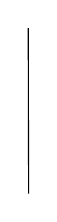
\begin{tikzpicture}[x=.25cm,y=.6cm]\draw (0,3.5)--(.02,0);\end{tikzpicture}}

\mspage{41}

